\documentclass[12pt]{extarticle}

\usepackage[MeX]{polski}
\usepackage[utf8]{inputenc}

\usepackage{times}
\usepackage{cite}
\usepackage{amsmath}
\usepackage{graphicx}
\usepackage{blindtext}
\usepackage{hyperref}
\usepackage{microtype}
\usepackage{afterpage}
\usepackage[dvipsnames]{xcolor}
\usepackage{listings}
\usepackage{chngcntr}
\usepackage[final]{pdfpages}

\lstset{frame=Trbl,numbers=left}

\renewcommand{\thefigure}{\thesection.\arabic{figure}}

\lstdefinelanguage{Java}{
  keywords={package, as, as?, typealias, this, super, val, var, fun, for, null, true, false, is, in, throw, return, break, continue, object, if, try, else, while, do, when, class, interface, enum, object, companion, override, public, private, get, set, import, abstract, vararg, expect, actual, where, suspend, data, internal, dynamic, final, by},
  keywordstyle=\color{NavyBlue}\bfseries,
  ndkeywords={@Deprecated, @JvmName, @JvmStatic, @JvmOverloads, @JvmField, @JvmSynthetic, Iterable, Int, Long, Integer, Short, Byte, Float, Double, String, Runnable, Array},
  ndkeywordstyle=\color{BurntOrange}\bfseries,
  emph={println, return@, forEach, map, mapNotNull, first, filter, firstOrNull, lazy, delegate},
  emphstyle={\color{OrangeRed}},
  identifierstyle=\color{black},
  sensitive=true,
  commentstyle=\color{gray}\ttfamily,
  comment=[l]{//},
  morecomment=[s]{/*}{*/},
  stringstyle=\color{ForestGreen}\ttfamily,
  morestring=[b]",
  morestring=[s]{"""*}{*"""},
}


\usepackage[left=3.5cm, right=2.5cm, top=2.5cm]{geometry}

\newcommand\tab[1][1cm]{\hspace*{#1}}

\linespread{1.5}

\author{Krzysztof Dragan}

\title{%
  Praca dyplomowa \\
  \large Aplikacja internetowa do wyszukiwania połączeń lotniczych}
  
\newcommand\blankpage{%
	\null
    \thispagestyle{empty}%
    \newpage}

\begin{document}

  \afterpage{\blankpage}
  
\includepdf[pages=-]{docs/strona_tytulowa.pdf}
  
  \afterpage{\blankpage}
  
\includepdf[pages=-]{docs/zadanie.pdf}

  \afterpage{\blankpage}
  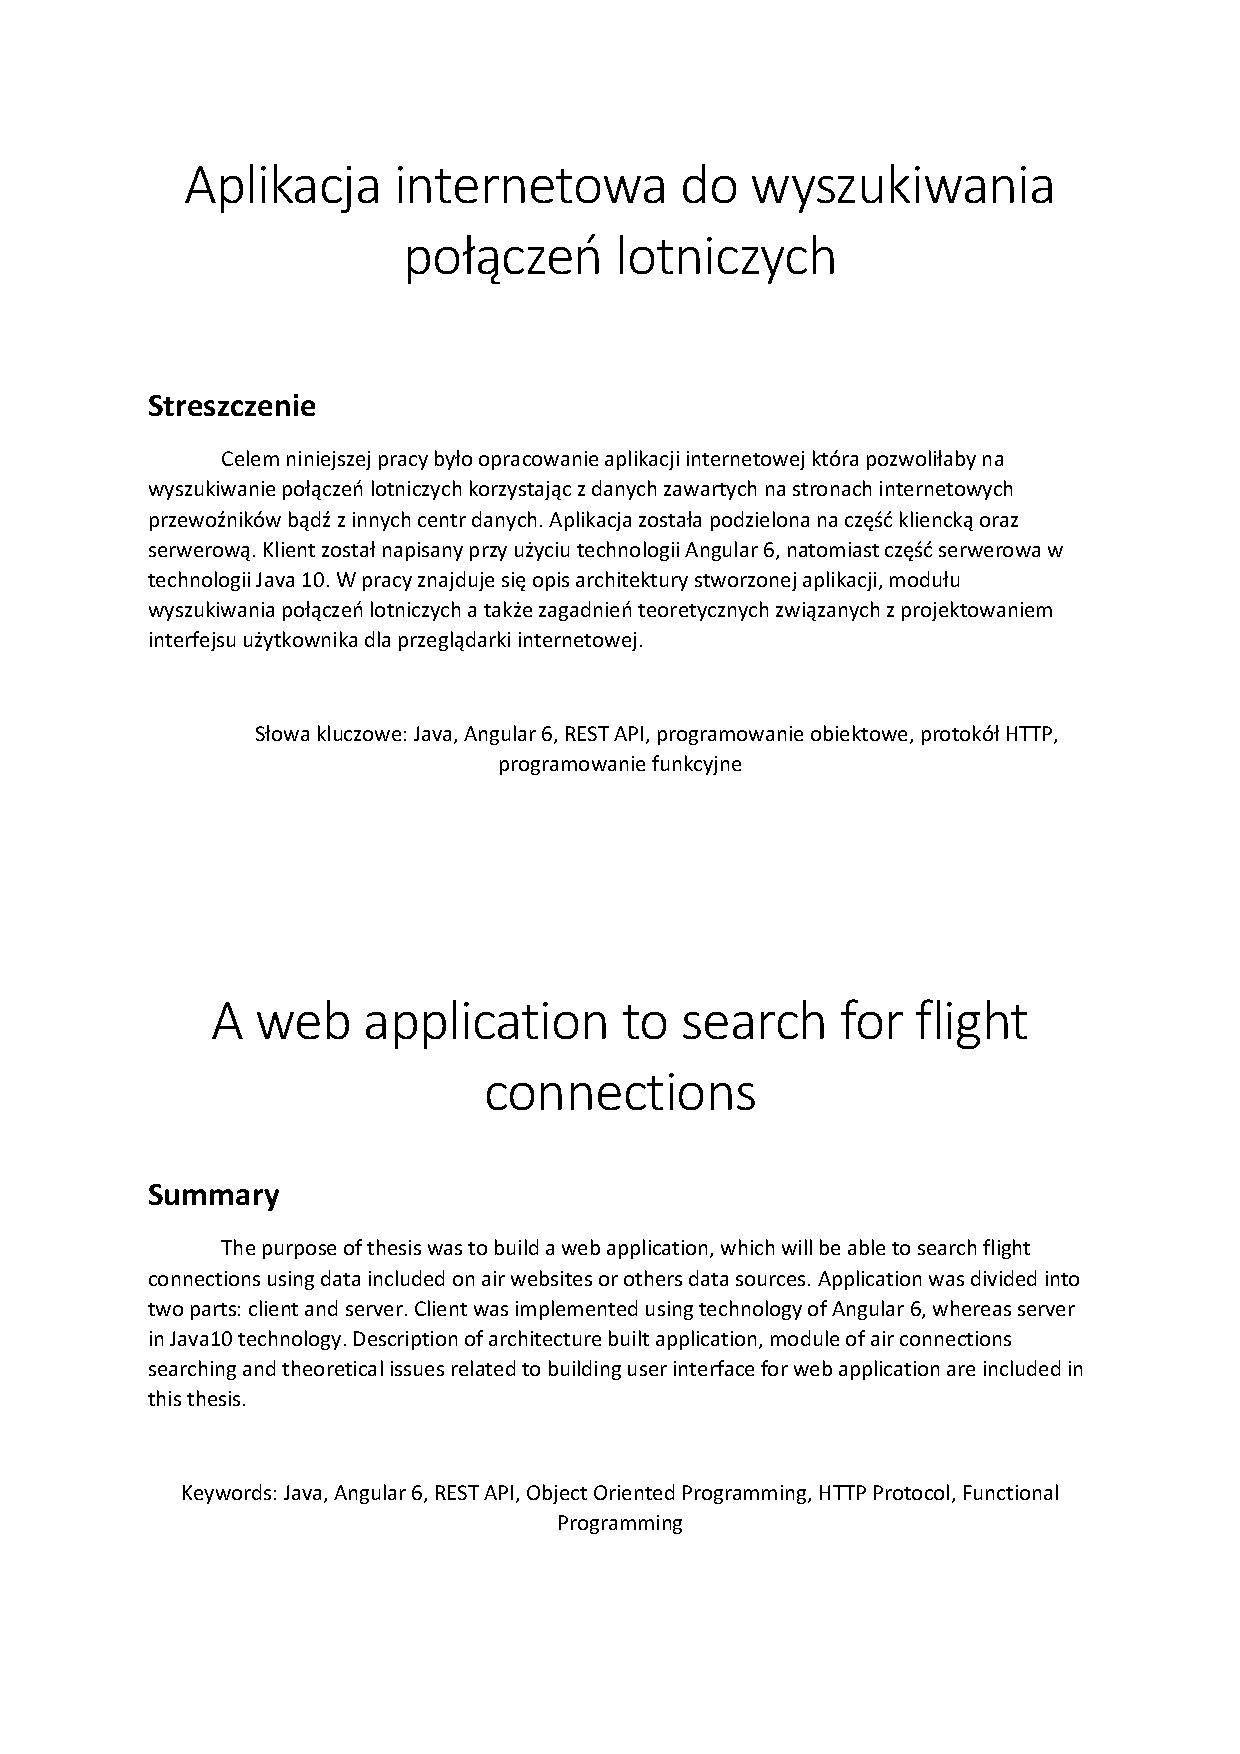
\includepdf[pages=-]{docs/streszczenie.pdf}

\newpage

\tableofcontents
\newpage
	
\section{Wstęp}
	\subsection{Example}
	\newpage
	
\section{Opis rozwiązywanego zagadnienia}
\subsection{Example}
\newpage

\section{Przegląd istniejących rozwiązań}
\subsection{Example}
\newpage


\section{Projekt aplikacji}
\subsection{Example}
\newpage


\section{Implementacja}
\subsection{Example}
\newpage


\section{Testy}
\subsection{Example}
\newpage


\section{Uwagi i wnioski}
	\subsection{Example}
	\newpage



\bibliography{Dokumentacja-blx}
\bibliographystyle{plain}

\end{document}
